\section{Introduction}
\label{sec:intro}

{ \color{red}
    Emphasize the hypothesis generation, remove references to OLAP}

Consider a data warehouse scenario: a database describes how a set of
\emph{measures} varies along several \emph{dimensions}. To work with this
database, analysts need a lot of prior knowledge: which dimensions and measures
they are interested in, where interesting patterns are hidden in the cube,
which dependencies among dimensions and measures exist, and much more.  Manual
exploration may expose some of this knowledge, but its success depends entirely
on chance and intuition. In contrast, we aim at a semi-automated exploration.
We want to assist the humans in understanding how measures are distributed,
where unexpected measures appear, and where interesting dependencies between
dimensions and measures arise.

We believe that automating query generation is essential to make analysts more
productive. Informations which are trivial for domain experts are not
necessarily so for data specialists. Besides, experts themselves may need
guidance. Consider for instance Figure \ref{intro}. The table shows a small
extract from a dataset of astronomical observations\footnote{This dataset come
from the LOFAR research programme, 21 May 2012, the Netherlands}. We want to
observe the \emph{brightness} of more than 100,000 sources, taken at different
times, frequency ranges and with different precisions. In total, there are more
than fifty dimensions. Even for an astronomer, this dataset cannot be
understood by intuition alone. We need intelligent tools to provide guidance.
The bottom picture illustrates what we expect from our query generation system:
a simpler low dimension view of dependent dimensions and measures.  Anyone can
quickly perceive bright regions.

\begin{figure}[t!]
\centering
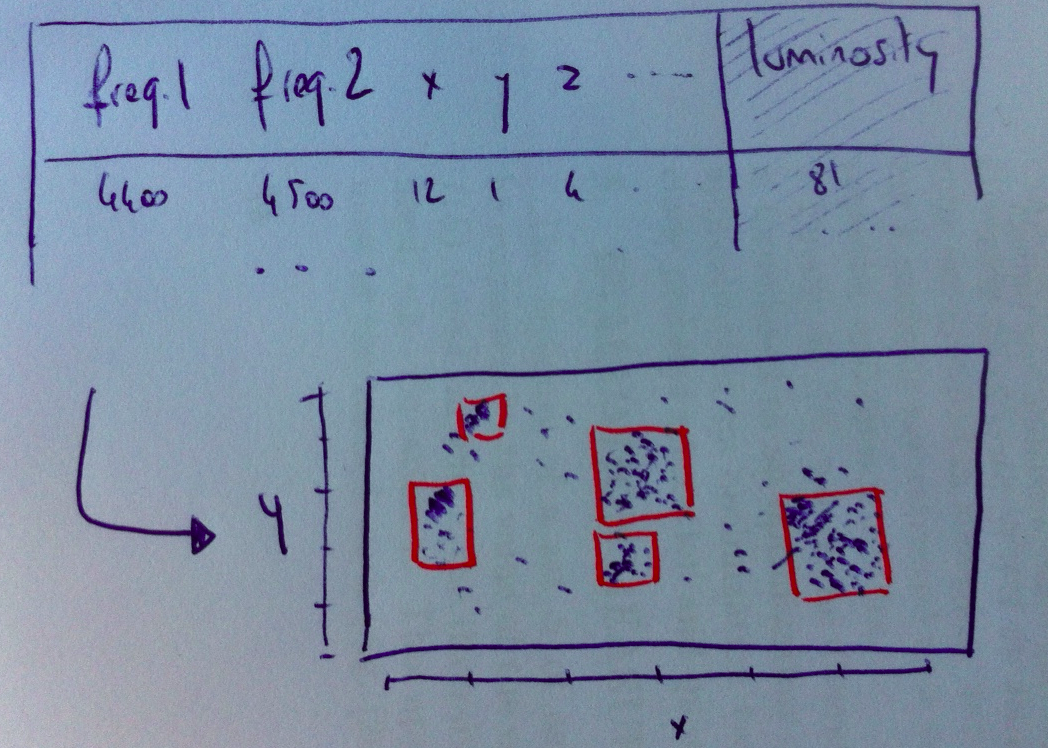
\includegraphics[width=0.8\columnwidth]{images/intro}
\caption{Revealing interesting regions}
\label{intro}
\end{figure}

Semi-automated exploration of data cubes is fundamentally challenging for two
reasons. The first reason is obvious: how do we recognize ``interesting''
queries?  The diversity of opinions in the literature is rather depressing.
What is interesting for a user can be extremely boring for another. The second
problem is practical.  Suppose that we had a universal measure of interest, how
could we explore the search space fast enough to find the interesting queries?

Many authors have proposed semi-automated (or discovery-driven) exploration
frameworks in the past. Typically, they introduce a fixed ``interestingness''
model, then the exploit the particularities of their model to speed up
computations.  For instance, a seminal work was presented by Sarawagi et al.
\cite{sarawagi1998discovery}. According to their paper, the most interesting
queries are the most ``surprising'' ones.  They suggest to build a (log-linear)
model over the data, and identify the largest deviations. More recently, Dash
et al.\cite{dash2008dynamic} proposed a facet selection method, also based on
surprise. Nevertheless, given the diversity of users and requirements, are
these interestingness models \emph{really} interesting?

In this paper, we introduce \textit{Claude}, a generic query generation
system. \emph{Claude lets users describe what they are looking for.
Given their input, it explores the database and reveals interesting OLAP views}.
Here is how it operates. First, the users assign a value to each tuple in
the database.  We call this value the \emph{target}. It can come from the raw
data (e.g., the brightness of light sources), a calculation (e.g., a
``surprise'' score from the litterature), or manual effort. Claude's job is to
present the ``big picture'': it explains how the target is distributed across
the database, and what influences it. To do so, it operates in two steps.
First, it explores the database for interesting projections. Then, for each
projection, it reveals ``remarkable'' areas. 

Making Claude efficient is a major challenge. We
introduce two algorithms.  The first one is exact and based on a systematic
level-wise search paradigm.  The second one is a much faster and based on a
relaxation of our model and a heuristic search.

\section{Preliminaries}

\subsection{Concepts}
\begin{figure}[t!]
\centering
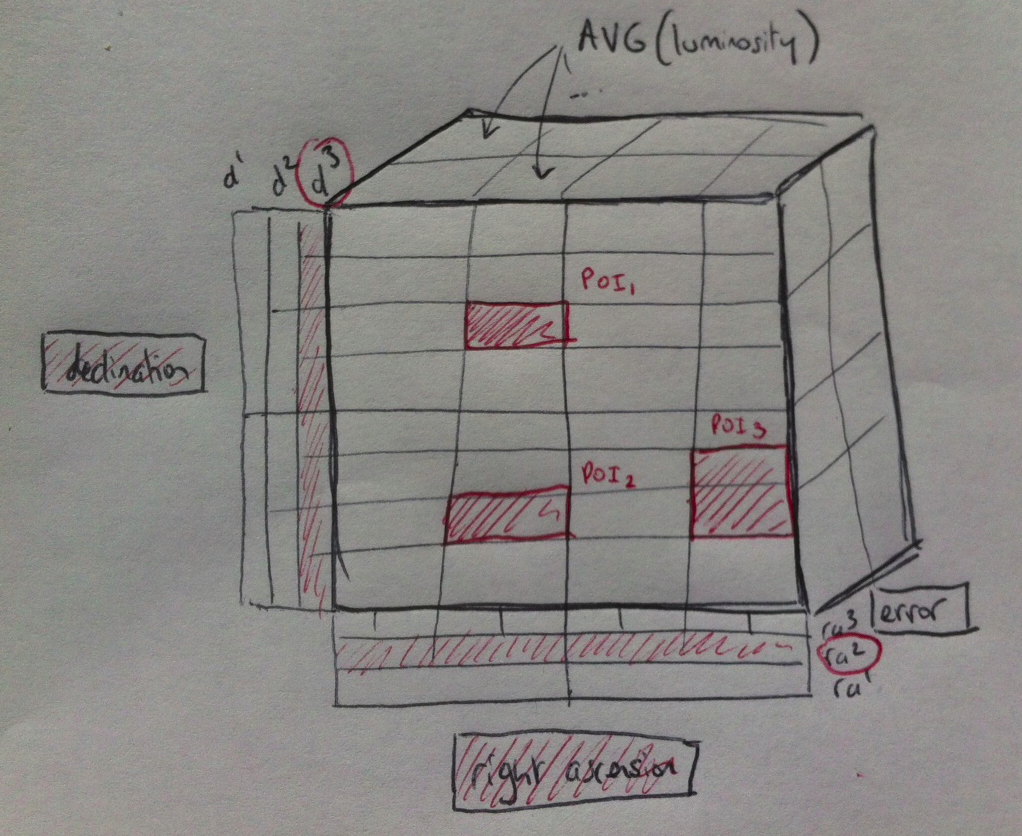
\includegraphics[width=0.9\columnwidth]{images/cube}
\caption{Example of recommendation}
\label{cube}
\end{figure}
We model the database as a large relation $DB$. This table contains two types
of columns: the dimensions $D_0, \ldots, D_d$ and a target column $T$. The
target column contains the target value for each tuple. Note that this view is
logical: we are oblivious to the physical structure of the data.  Claude's aim
is to generate a set of \textbf{explanations}.  An explanation contains two
elements: a \textbf{view} and several \textbf{points of interest} (POI). A view
is an ``informative'' set of dimensions, on which we project the data.  A point of
interest is a selection over this view. It contains tuples for which the target
has a ``remarkable'' distribution.

We illustrate these concepts with Figure \ref{cube}. Our example database
describes light sources.  It contains three dimensions: \texttt{right
ascension}, \texttt{declination} and \texttt{error}. The first two describe a
source's position. The third one describes the measurement errors. For each
tuple, we target the value of the column \texttt{brightness}. Claude's output
is highlighted in red. It contains a view based on \texttt{right ascension},
and \texttt{declination}. We see that the view is a SQL query with the
following structure:
\begin{verbatim}
SELECT   D1, ... , Dn , AVG(T)
FROM     DB 
GROUPBY  D1, ... , Dn
\end{verbatim}
The $n$ distinct variables $\texttt{D1} \ldots \texttt{Dn}$ define the view. Once
Claude has chosen a view, it must explain \emph{why} it has chosen this view.
This is the role of POIs. In Figure \ref{cube}, Claude suggests three POIs. We
can express them in SQL as follows:
\begin{verbatim}
SELECT   AVG(T)
FROM     DB
WHERE    D1 BETWEEN l1 AND h1
 AND     ...
 AND     Dn BETWEEN ln AND ln
\end{verbatim}
The POIs are defined by the ranges $\texttt{[l1,h1]}, \dots \texttt{[ln,hn]}$.


\subsection{Informative explanations}
\label{sec:infor}
\begin{figure}[t!]
\centering
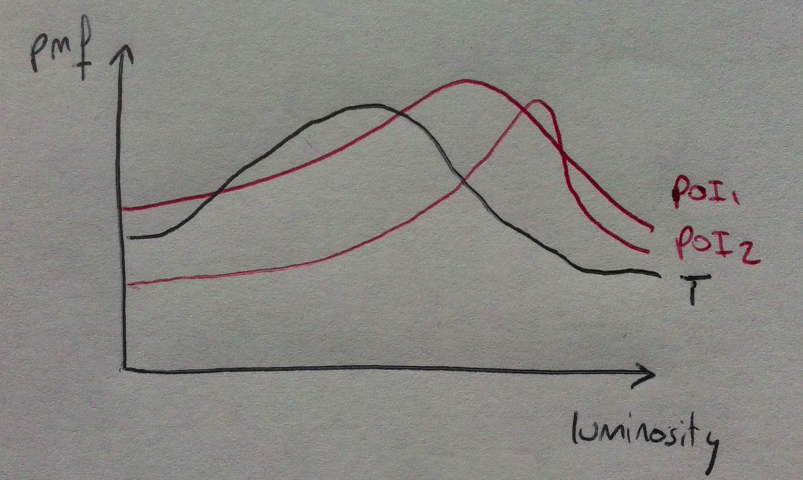
\includegraphics[width=\columnwidth]{images/poi}
\caption{The POIs have unusual distributions}
\label{poi}
\end{figure}

We defined Claude's search space: we want to suggest views and POIs. We now
present how the target helps us recognize the ``interesting'' ones. 

First let's explain how to choose the views. A set of columns is informative if
it is somehow related to the target: if we filter the data on these columns,
the target value changes.  We model this relationship with statistical
dependency. We represent each  dimension $D_k$ by a random variable $\rv{D}_k$.
We model the target with a random variable $\rv{T}$.  A view is interesting if
there exists some statistical dependency between its columns and the target. We
formalize this statement with Mutual Information \cite{cover2012elements}:

\begin{definition}
Consider a view $V = \{D_1, \ldots, D_n\}$, and the target column $T$.  Let
$I$ denote the \emph{Mutual Information} between two random variables. We
define the \textbf{strength} of $V$ as follows:
\[\sigma(V) = I(\rv{D}_1, \ldots, \rv{D}_n ; \rv{T})\]
\end{definition}

{\color{red}
Detail what the MI is, how to compute, etc...
}

Claude seeks variables which are \emph{jointly depdendent} to the target. We
measure dependency with the mutual information, because this quantity is
general (correlation is only one type of dependency).

The next step is to extract the POIs. The POIs contain tuples for which the
measure have an ``unusual'' distribution compared to the rest of the database.
Consider Figure \ref{poi}. The curves show the probability mass function of the
brightness for three sets of tuples: the whole database, $POI_1$ and $POI_2$.
The sets $POI_1$ and $POI_2$ come from the view \texttt{right ascension -
declination} in Figure \ref{cube}. We observe that they deviate from $DB$.
They illustrate how right ascension and declination can influence brightness.
We quantify this observation with the Kullback-Leibler divergence:

\begin{definition}
Consider a range $R = [l_1, h_1] \times \ldots \times [l_n, h_n]$. 
The random variable $\rv{T}_R$ describes the target for
the tuples in $R$, and $\Pr(\rv{T}_R)$ its distribution.
We define the \textbf{divergence} of the range $R$ as follows: 
\[\delta(R) = KL \big( \Pr(\rv{T}) \| \Pr(\rv{T_R})  \big)\]
\end{definition}

The Kullback-Leibler divergence measures the difference between two probability
distributions. Our function $\delta$ grows when a range has unsual target
values, it decreases otherwise. It does not target specifically high or low
values. It seeks \emph{any} type of deviation from the target's global
distribution.  Note that divergence is tightly related to strength:

\begin{lemma}
Let $V$ denote a view. We create a grid over $V$ by discretizing its
columns. The variable $\rv{R}$ describes a random cell.  We observe the
following relationship:
\[
    \sigma(V) = \mathbb{E}_{\rv{R}} \{ \delta(\rv{R}) \}
\]
\end{lemma}

\begin{proof}
Let $\rv{V}$ represent the joint distribution $\rv{D}_1, \ldots, \rv{D}_n$.
We have $\sigma(V) = I(\rv{V},\rv{T})$.
By definition of the Kullback-Leibler divergence, we have: 
$I(\rv{V},\rv{T}) = $ $\mathbb{E}_{\rv{V}} \{ KL( \Pr(\rv{T} | \rv{V}) \|$ $ \Pr(\rv{T}) ) \}$
As the data is discretized, $\rv{V}$ and $\rv{R}$ are equivalent. Also,
for any bin $R$, $\Pr(\rv{T} | \rv{V} = R)$ is equivalent to
$\Pr(\rv{T}_R)$. We derive the lemma.
\end{proof}


This lemma is simple but powerful. It shows that strength and divergence are
``two sides of the same coin'': the strength of a view equals exactly the
average divergence of its bins. We use the terms strength and
deviation interchangeably to characterize an \emph{explanation} (recall that a
explanation contains both the view and its POIs).

\begin{definition}
Let $S=(\{ D_1, \ldots, D_n\}, \{R_1, \ldots, R_r\})$ describe an explanation . The
\textbf{strength} (or \textbf{divergence}) of $S$ equals the strength
of its view.
\end{definition}

We are now ready to formulate our problem.

\begin{problem}
Consider a dataset $DB$, a target column $T$ and a triplet $(q, n, r)$. Find
the top $q$ strongest explanations, with $n$ variables and $r$ POIs.
\end{problem}

To solve this problem, Claude operates in two steps. First, it detects $q$
strong sets of columns.  We call this step \emph{column search}.  Then comes
the \emph{POI dectection} step: for each view we extract $r$ POIs. In practice,
our top $q$ strategy can generate redundancy. We tackle this problem with an
optional \emph{refinment} step.

\section{Column selection}
\label{sec:colum}

{\color{red} 
This section requires some reordering.
\begin{itemize}
    \item Introduce Lemma 2, and the idea to search for columns greedily
    \item Present the exact approach
    \item Present the approximation
\end{itemize}
Also, the description of the approximation should be deepened.
}

The aim of this phase is identify the $q$ strongest sets of variables. From
here on, we use the notations $D_i$ and $\rv{D}_i$ interchangeably - we can use
the context to distinguish database columns and random variables.

\subsection{Base algorithm}
\begin{figure}[t!]
\centering
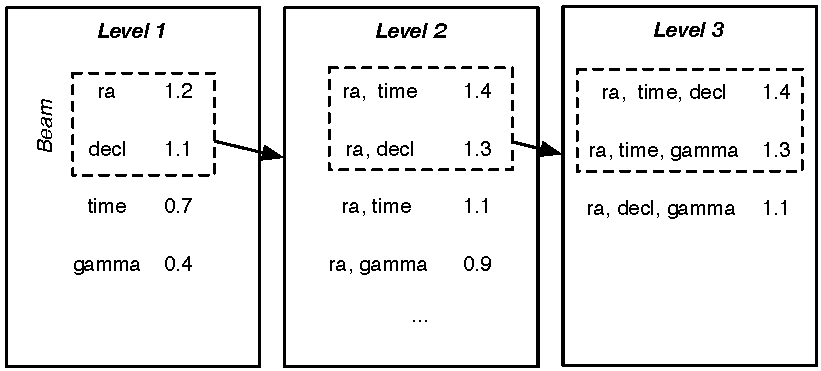
\includegraphics[width=0.8\columnwidth]{images/beam-search}
\caption{Example of Beam Search, with a beam size of 2}
\label{pic:beam-search}
\end{figure}

To recommend views, Claude must find the best sets of at most $n$ variables.
The search space of this problen grows exponentially with $n$: from a database
with $d$ variable, we can generate $\sum_{i \leq n} \binom{d}{i}$ combinations.
Besides, there is to our knowledge no bound which would allow us to prune the
search space efficiently. 

We propose to use level-wise search. To initialise the algorithm, we compute
the strength of each variable separately (we compute $\sigma(D_i) = I(D_i;
T)$). We order the candidates, and keep the top $b$ variables. We call this set
the \emph{beam}. We then form new candidates by appending each variable of the
database to each variable in the beam. We obtain views with two columns. We
compute the best $b$ results and update the beam. The procedure is repeated
until the beam contains views with $n$ variables. We illustrate the procedure
in Figure \ref{pic:beam-search}.

\begin{figure}[t!]
\centering
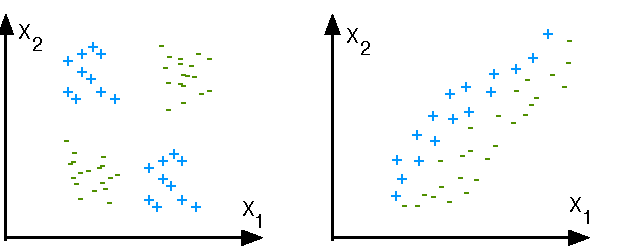
\includegraphics[width=0.8\columnwidth]{images/strength-jump}
\caption{Limit cases of the beam search strategy. The variables $var1$ and
$var2$ represent two dimensions. The symbol and color of the plots represent
the value of the target class. }
\label{pic:strength-jump}
\end{figure}
Thanks to our beam strategy, we avoid exploring an exponentially large search
space. Instead, we compute the strengths of at at most $n.b$ settings.
Unfortunately, this strategy induces an accuracy penalty: if the beam is too
small, we may miss some good candidates. This is a consequence of the following
observation: a set of columns which is outside the top $q$ candidates at step
$i$, could very well appear in the top $q$ at step $i+1$. Consider for instance
the two classic scenarios pictured in Figure \ref{pic:strength-jump}. The
dimensions $var1$ and $var2$ taken in isolation are weak: we can infer no
useful information about the target from either of them. However, their
combination is very interesting.  This observation is reflected by the
strength: the views $\{var1\}$ and $\{var2\}$ have a very poor strength, but
$\{var1, var2\}$ is an excellent candidate. If use a beam search strategy, we
may discard  $\{var1\}$ and $\{var2\}$ early because they have a low score.
This would be a mistake, because we lose the opportunity to discover $\{var1,
var2\}$.

\subsection{Approximating the View Strength}
\label{sec:approx}


The Beam Search aslgorithm gives us a convenient way to find good views.
Through the size of the beam, we can find a compromise between execution time
and accuracy.  Nevertheless, the algorithm is still too heavy for an
interactive application. For each candidate, it computes the mutual information
between all the variables of the view and the target, which involves heavy grouping
operations. Our solution is to \emph{approximate} the strength of the views
during the iterations of the algorithm. Then, we use exact calculations for the
final ranking.

To present our approximation scheme, we must first describe how a
view is impacted when we add a column to it.

\begin{lemma}\label{lem:chain}
Consider a view $V = \{D_1, \ldots, D_i\}$, and a target $T$.
For any column $D_{i+1}$: 
$$
\sigma(V \cup \{D_{i+1}\}) =  \sigma(V) + I(D_{i+1} ; T | D_1 , \ldots, D_i)
 $$
\end{lemma}
\begin{proof}
This lemma is a direct consequence of the Mutual Information's chain rule
\cite{cover2012elements}.
\end{proof}

This lemma describes how much a view improves if we append a new dimension.
For any random variables $X,Y,Z$, the notation $I(X;Y|Z)$ expresses the
\emph{conditional mutual information}. It describes the dependency between $X$
and $Y$, \emph{given $Z$}. The influence of $Z$ can go either way: it can
weaken or strengthen the relationship between $X$ and $Y$. In any case, it is
positive or null, and it is bounded by the entropy of $X$ and $Y$.

In practive, computing $ I(D_{i+1} ; T | D_1 , \ldots, D_i)$ is not less
expensive than calculating the strength of $\{D_1, \ldots, D_{i+1}\}$ directly.
But we can use the following approximation:
\[
\begin{split}
    \sigma(V \cup \{D_{n+1}\}) & = \sigma(V)   + I(D_{n+1} ; T | D_0, \ldots, D_{n})\\
                           & \approx \sigma(V) + I(D_{n+1} ; T | D_{i})
\text{ for } D_i \in V
\end{split}
\]

The idea behind this approximation is naive: we assume that $I(D_{n+1} ; T |
D_0, \ldots, D_{n}) \approx I(D_{n+1} ; T | D_{i})$. We ignore the high order
dependencies. Thanks to this assumption, we can compute the strength of a view
much faster.  Consider a directed graph in which each vertex represents a
variables $D_i$. Each edge $(D_i, D_{i+1})$ has a a weight $ I(D_{i+1} ; T |
D_{i})$.  We call this graph \emph{co-dependency} graph.  To compute the
approximate strength of ${D_0, \ldots, D_i}$, we build a spanning tree which
covers all the vertices of the view, and sum the weights of the edges.

In most cases, we can build several different spanning trees with different
weights. Which one should we use? We could use two variants. An
\emph{optimisic} approximation $\sigma_+ $ would consider the \emph{maximum}
spanning tree.  A \emph{pessimistic} approximation $\sigma_- $ would use the
weight of the \emph{minimum} spanning tree. For the rest of this paper, we will
only consider the latter aleternative. 

We now present a faster version of our view search algorithm.  We operate in
two steps. First, we compute the strength of every column and every couple of
columns.  This gives us a first set of candidates, and we can derive the
co-dependency graph using the fact that $I(D_{j} ; T | D_i) = \sigma(D_i ;
D_{j}) - \sigma(D_i)$.  Then, we run Beam Search as previously, but with the
approximate strength computation.  To append the variable $D_i$ to the view
$V$, we list every edge which connects  $D_i$ to the columns of $V$. We
identify the lightest one and add the value of its weight to $\sigma(V)$.  

This algorithm is much faster because it spares us expensive database
operations. Instead, we perform computations on a graph with $d$ nodes.  To
save some accuracy, we use the exact version of the view strength for the final
top $q$ ranking.

\section{Detecting Points Of Interest}
\label{sec:detec}

During this phase, we find the $r$ most divergent regions for each view.
Fortunatly, this task is an instance of a known Data Mining problem,
\emph{Subgroup Discovery} \cite{klosgen1996explora}\cite{wrobel1997algorithm}.
The aim of Subgroup Discovery is to identify sets for which the target value
maximizes a user-defined quality measure. To solve our problem, we instantiate
the quality measure with the divergence.

In principle, we could use any efficient algorithm from the Subgroup Discovery
litterature.  We propose to reuse the beam Search strategy from the previous
section, but to explore \emph{tuples} instead of columns. We bin the data in a
coarse manner and get a first set of $b$ cells. We then refine these cells with
a thinner binning, etc...

As mentioned in the Subgroup Discovery litterature \cite{van2011non}, our
divergence score has a drawback: it favours smaller groups.  Therefore, Beam
Search may converge very late or not at all.  A practical
solution is to alter the model to take the size into account. Let $R$
represents a range with cover $|R|$, and $|V|$ represent the number of tuples
in the view. We use the \emph{weighted} deviation $\delta_w(R) = |R|/|V| \times
\delta(R)$. This new score introduces a penalty for small POIs.


\section{Improving the Diversity of the Views}

{ \color{red} This section should go. Instead, replace it with a few mentions
to deduplication in the previous section and/or in the experiments}

As Claude is based on a top-k approach, its output may be redundant: the views
may be very similar to each other.  Some users prefer small but diverse sets of
suggestions.  We tackle this problem with compression techniques from the
frequent petterns literature. For instance, the Krimp algorithm is an
established strategy, based on the Minimum Description Length principle
\cite{vreeken2011krimp}. Another approach would be to cluster the views, and
return one representative view per cluster.


\section{Experiments}

\begin{table}
    \centering
    \small
    \begin{tabular}{r c c c c} 
        \hline
        Dataset & Columns & Rows & \#Views & \#Variables\\
        \hline
        MuskMolecules & 167 & 6,600 & 22 & 18\\
        Crime & 128 & 1,996 & 20 & 17\\
        BreastCancer & 34 & 200 & 10 & 13\\
        PenDigits & 17 & 7,496 & 9 & 10\\
        BankMarketing & 17 & 45,213 & 11& 8\\
        LetterRecog & 16 & 20,000 & 10 & 12\\
        USCensus & 14 & 32,578 & 10 & 7\\
        MAGICTelescope & 11 & 19,022 & 1 & 11\\
        \hline
    \end{tabular}
    \caption{Characteristics of the datasets. The last two columns are used for
    comparison with 4S, as explained in \ref{sec:exp-view-selection}.}
    \label{tab:datasets}
\end{table}

\subsection{Detailed Example: Crimes in the US}

\begin{table}[t]
  \centering
  \small
  \rowcolors{2}{gray!25}{white}
  \begin{tabulary}{\columnwidth}{L c}
    \hline
    View & Score (normalized)\\
    \hline
    Police.Overtime, Pct.Vacant.Boarded, Pct.Race.White & 0.51\\
    Pct.Families.2.Parents, Pct.Race.White, Police.Requests.Per.Officer & 0.49\\
    Pct.Police.White, Pct.Police.Minority, Pct.Vacant.House.Boarded& 0.37\\
    Pct.Empl.Profes.Services, Pct.Empl.Manual, Pct.Police.On.Patrol & 0.37\\
    Pct.Retired, Pct.Use.Public.Transports, Pct.Police.On.Patrol& 0.35 \\
    Pct.Recently.Moved, Population.Density, Police.Cars & 0.34 \\
    \hline
\end{tabulary}
    \caption{Example of views generated by Claude for the US Crime dataset.}
    \label{tab:crime_views}
\end{table}

\begin{figure}[t!]
    \centering
    \begin{subfigure}[b]{0.42\columnwidth}
    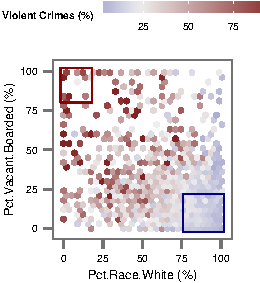
\includegraphics[width=\textwidth]{plots/crime1}
    \end{subfigure}
    \begin{subfigure}[b]{0.42\columnwidth}
    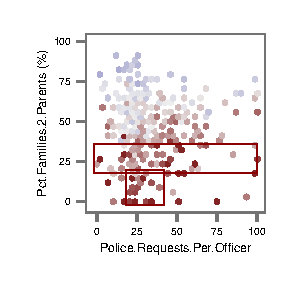
\includegraphics[width=\textwidth]{plots/crime2}
    \end{subfigure}

    \begin{subfigure}[b]{0.42\columnwidth}
    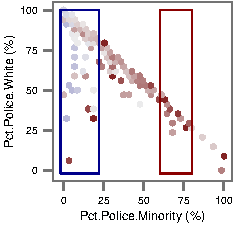
\includegraphics[width=\textwidth]{plots/crime3}
    \end{subfigure}
    \begin{subfigure}[b]{0.42\columnwidth}
    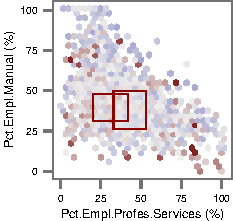
\includegraphics[width=\textwidth]{plots/crime4}
    \end{subfigure}
    
    \begin{subfigure}[b]{0.42\columnwidth}
    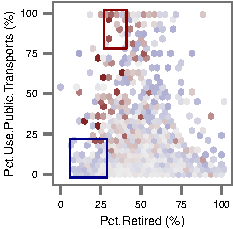
\includegraphics[width=\textwidth]{plots/crime5}
    \end{subfigure}
    \begin{subfigure}[b]{0.42\columnwidth}
    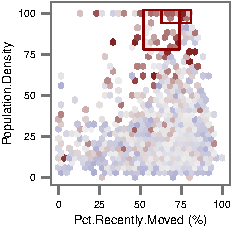
\includegraphics[width=\textwidth]{plots/crime6}
    \end{subfigure}
\caption{Heatmaps of the US Crime Dataset, based on Claude's output. Each box
represents a Point of Interest.}
\label{pic:crime_charts}
\end{figure}


\subsection{View Score and Prediction}

\begin{figure}[t!]
\centering
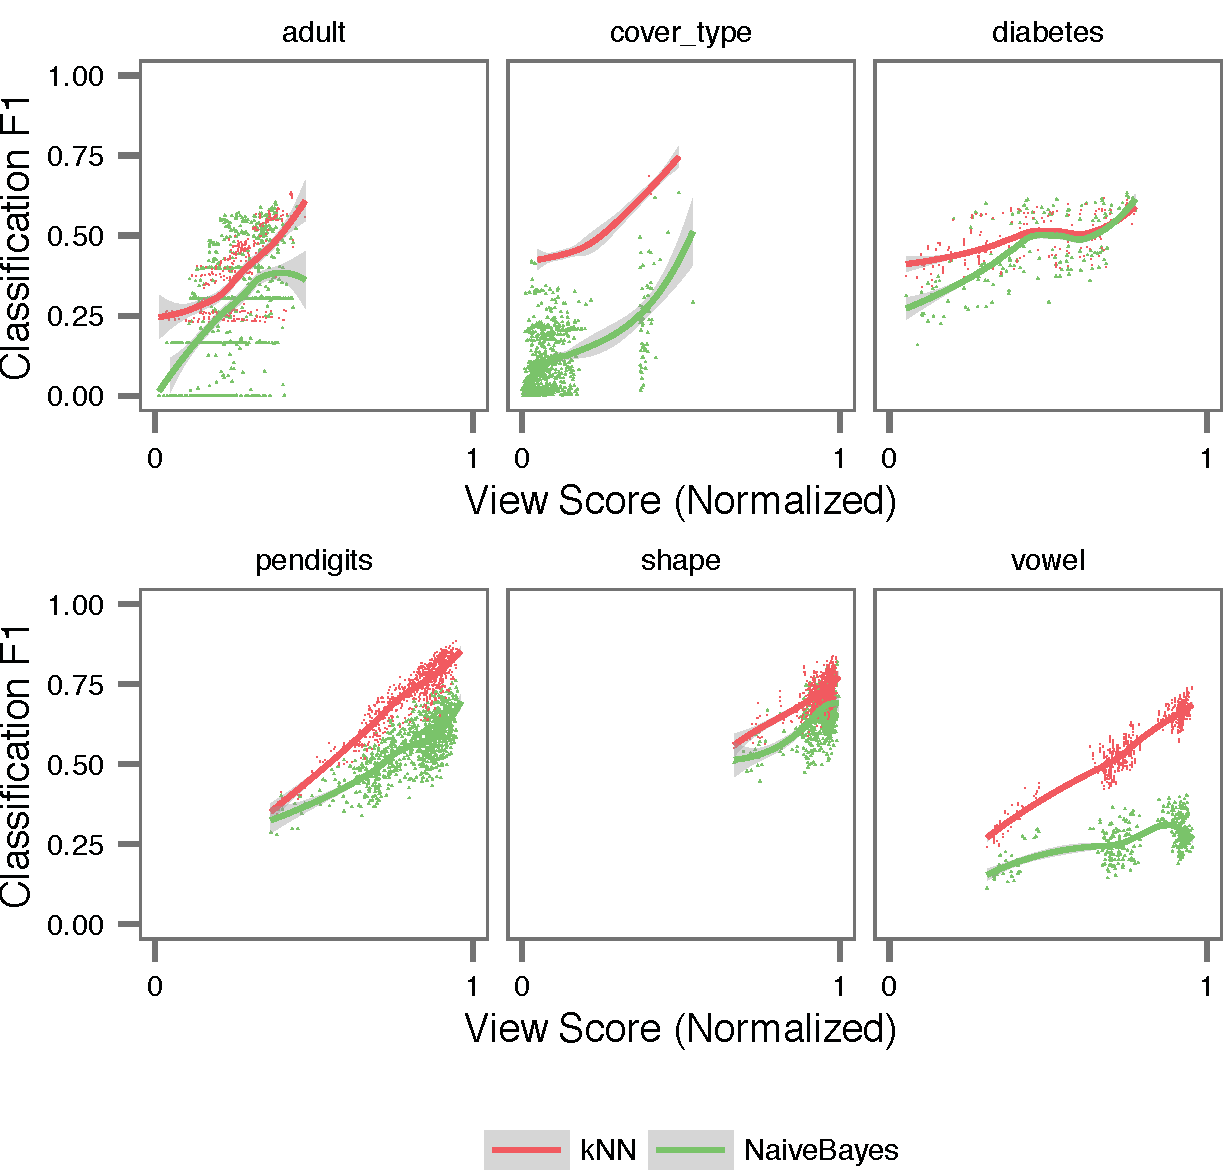
\includegraphics[width=\columnwidth]{plots/compare-strength-f1}
\caption{Strength vs. Classification accuracy for 500 random views. The blue
    and red lines represent local regressions, computed on a sliding window of
    80 points. The grey shades around the lines represent 90\% confidence
    intervals.}
\label{pic:strength-vs-f1}
\end{figure}

\subsection{View Selection}
\label{sec:exp-view-selection}

\begin{figure*}[t!]
\centering
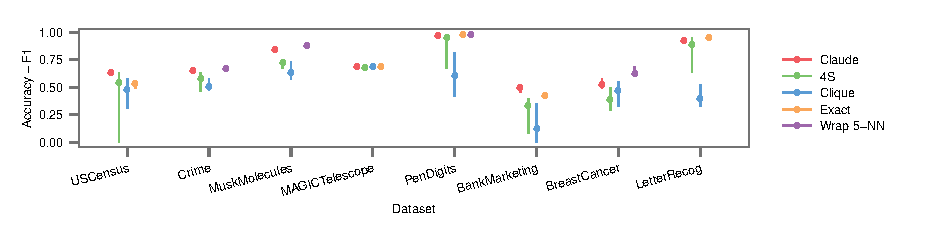
\includegraphics[width=2\columnwidth]{plots/view-scores}
\caption{Performance of the View Selection algorithms. For each data set, we
    generate $q$ views, train a 5-NN classifier over the columns of each view
    and report the classification accuracy (F1). The points represent
    median scores, the bars represent minimum and maximum scores.} 
\label{pic:column-select-score}
\end{figure*}

\begin{figure*}[t!]
\centering
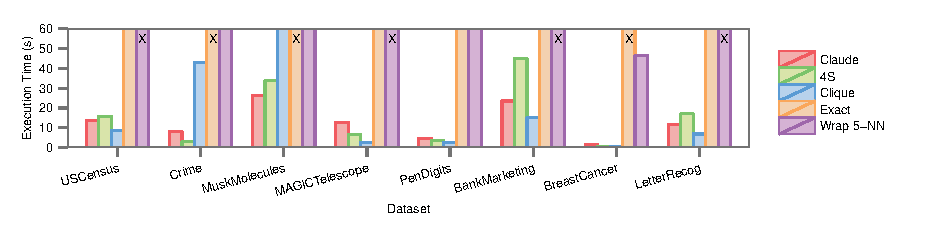
\includegraphics[width=2\columnwidth]{plots/view-times}
\caption{Execution time of the View Selection algorithms. A \texttt{X} symbol
indicates that the experiment did not finish within 3,600 seconds.}
\label{pic:column-select-time}
\end{figure*}

\begin{figure}[t!]
\centering
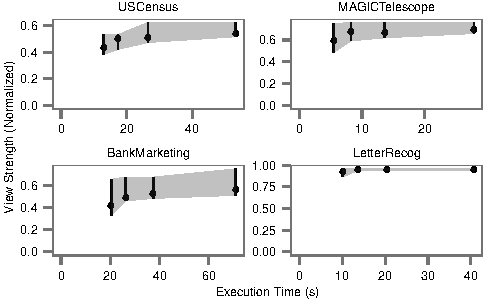
\includegraphics[width=\columnwidth]{plots/view-vary-beam}
\caption{.}
\label{pic:view-beam}
\end{figure}

\begin{figure}[t!]
\centering
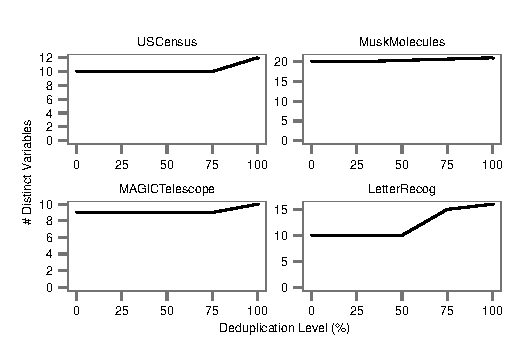
\includegraphics[width=\columnwidth]{plots/view-vary-diversification}
\caption{.}
\label{pic:view-diversification}
\end{figure}


\subsection{POI Detection}

\begin{figure*}[t!]
\centering
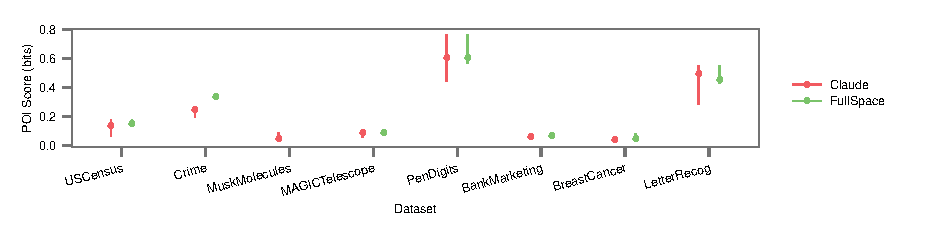
\includegraphics[width=2\columnwidth]{plots/POI-score}
\caption{Quality of the POIs.}
\label{pic:POI-quali}
\end{figure*}

\begin{figure*}[t!]
\centering
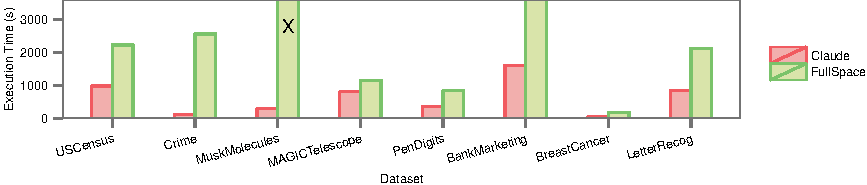
\includegraphics[width=2\columnwidth]{plots/POI-timing}
\caption{}
\label{pic:POI-time}
\end{figure*}

\section{Related Work}
Our work is inspired by both database research and machine learning. On the
database side, Claude is related to the \emph{query recommendation} problem:
how to automatically generate interesting SQL queries for a given database? On
the machine learning side, our work is based on \emph{feature selection}, e.g.,
how to select variables for a given inference problem, and \emph{subgroup
discovery}, e.g., how to find the tuples which maximize a particular score
function.

\textbf{Query Recommendation.} We identify two types of recommendation systems:
\emph{human-driven} approaches and \emph{data-driven} approaches. Human-driven
systems learn from user feedback. For instance, Chatzopoulou et al. propose to
make recommendations from query logs, similarly to search engines
\cite{chatzopoulou2009query}. More recently, authors have proposed interactive
exploration systems, where a recommendation system ``guides'' the user through
the database. In Explore-by-Example, the system infers queries from examples
provided by the user \cite{dimitriadou2014explore}. With Charles, the engine
decomposes large queries into smaller ones \cite{sellam2013meet}. Sarawagi's
method builds a maximum entropy model over the database from the user's history 
\cite{sarawagi2000user}. Bonifati et al. propose a similar method to recomend
joins \cite{bonifati2014interactive}.  Claude competes with neither of these
approaches, since it uses the content of the database only.

Our work is closer data-driven data recommendation, in which the system makes
recommendations based on the content of the data. The general idea is to build
a statistical model of the database, and find regions which behave
unexpectedly. Sarawagi et al. have published seminal work on this topic for
OLAP cubes \cite{sarawagi1998discovery}. Their system highlights sequences of
drill-in operations which lead to ``surprising data'', e.g., tuples which
differ from their neighbourhood. It requires that the data is organized in an
OLAP cube (with hierchical dimensions), it supposes that the users know which
variables to use, and it seeks thin-grained deviations. Oppositely, our system
uses regular tables, it recommends views (not only selections) and it seeks
large trends. More recently, Dash et al. have proposed a method to reveal
surprising subsets in a faceted search context \cite{dash2008dynamic}. This
method is related to Claude, but it targets document search, it does not
recommend views.


\textbf{Feature Selection, Subspace Search.} Chosing which variables to use for
classification or regression is a crucial problem, for which dozens of methods
were proposed \cite{guyon2003introduction}. A typical feature selection
algorithm outputs one set of variables on which a certain predictor performs
optimally. Our objective is different: we seek several, small sets of variables,
simple enough to be interepreted by a humans. Claude is halfway between
inference and exploration.

On the unsupervised learning side, our work is close to subspace search. The
idea is detect subspaces where the data is clustered distinctly
\cite{keller2012hics,nguyen20134s}. We compare Claude to state-of-the-art
methods in our Experiments section.

\textbf{Subgroup Discovery.}

\section{Conclusion}
